% Options for packages loaded elsewhere
\PassOptionsToPackage{unicode}{hyperref}
\PassOptionsToPackage{hyphens}{url}
\PassOptionsToPackage{dvipsnames,svgnames,x11names}{xcolor}
%
\documentclass[
  letterpaper,
  DIV=11,
  numbers=noendperiod]{scrartcl}

\usepackage{amsmath,amssymb}
\usepackage{iftex}
\ifPDFTeX
  \usepackage[T1]{fontenc}
  \usepackage[utf8]{inputenc}
  \usepackage{textcomp} % provide euro and other symbols
\else % if luatex or xetex
  \usepackage{unicode-math}
  \defaultfontfeatures{Scale=MatchLowercase}
  \defaultfontfeatures[\rmfamily]{Ligatures=TeX,Scale=1}
\fi
\usepackage{lmodern}
\ifPDFTeX\else  
    % xetex/luatex font selection
\fi
% Use upquote if available, for straight quotes in verbatim environments
\IfFileExists{upquote.sty}{\usepackage{upquote}}{}
\IfFileExists{microtype.sty}{% use microtype if available
  \usepackage[]{microtype}
  \UseMicrotypeSet[protrusion]{basicmath} % disable protrusion for tt fonts
}{}
\makeatletter
\@ifundefined{KOMAClassName}{% if non-KOMA class
  \IfFileExists{parskip.sty}{%
    \usepackage{parskip}
  }{% else
    \setlength{\parindent}{0pt}
    \setlength{\parskip}{6pt plus 2pt minus 1pt}}
}{% if KOMA class
  \KOMAoptions{parskip=half}}
\makeatother
\usepackage{xcolor}
\setlength{\emergencystretch}{3em} % prevent overfull lines
\setcounter{secnumdepth}{-\maxdimen} % remove section numbering
% Make \paragraph and \subparagraph free-standing
\makeatletter
\ifx\paragraph\undefined\else
  \let\oldparagraph\paragraph
  \renewcommand{\paragraph}{
    \@ifstar
      \xxxParagraphStar
      \xxxParagraphNoStar
  }
  \newcommand{\xxxParagraphStar}[1]{\oldparagraph*{#1}\mbox{}}
  \newcommand{\xxxParagraphNoStar}[1]{\oldparagraph{#1}\mbox{}}
\fi
\ifx\subparagraph\undefined\else
  \let\oldsubparagraph\subparagraph
  \renewcommand{\subparagraph}{
    \@ifstar
      \xxxSubParagraphStar
      \xxxSubParagraphNoStar
  }
  \newcommand{\xxxSubParagraphStar}[1]{\oldsubparagraph*{#1}\mbox{}}
  \newcommand{\xxxSubParagraphNoStar}[1]{\oldsubparagraph{#1}\mbox{}}
\fi
\makeatother


\providecommand{\tightlist}{%
  \setlength{\itemsep}{0pt}\setlength{\parskip}{0pt}}\usepackage{longtable,booktabs,array}
\usepackage{calc} % for calculating minipage widths
% Correct order of tables after \paragraph or \subparagraph
\usepackage{etoolbox}
\makeatletter
\patchcmd\longtable{\par}{\if@noskipsec\mbox{}\fi\par}{}{}
\makeatother
% Allow footnotes in longtable head/foot
\IfFileExists{footnotehyper.sty}{\usepackage{footnotehyper}}{\usepackage{footnote}}
\makesavenoteenv{longtable}
\usepackage{graphicx}
\makeatletter
\newsavebox\pandoc@box
\newcommand*\pandocbounded[1]{% scales image to fit in text height/width
  \sbox\pandoc@box{#1}%
  \Gscale@div\@tempa{\textheight}{\dimexpr\ht\pandoc@box+\dp\pandoc@box\relax}%
  \Gscale@div\@tempb{\linewidth}{\wd\pandoc@box}%
  \ifdim\@tempb\p@<\@tempa\p@\let\@tempa\@tempb\fi% select the smaller of both
  \ifdim\@tempa\p@<\p@\scalebox{\@tempa}{\usebox\pandoc@box}%
  \else\usebox{\pandoc@box}%
  \fi%
}
% Set default figure placement to htbp
\def\fps@figure{htbp}
\makeatother

\KOMAoption{captions}{tableheading}
\makeatletter
\@ifpackageloaded{caption}{}{\usepackage{caption}}
\AtBeginDocument{%
\ifdefined\contentsname
  \renewcommand*\contentsname{Table of contents}
\else
  \newcommand\contentsname{Table of contents}
\fi
\ifdefined\listfigurename
  \renewcommand*\listfigurename{List of Figures}
\else
  \newcommand\listfigurename{List of Figures}
\fi
\ifdefined\listtablename
  \renewcommand*\listtablename{List of Tables}
\else
  \newcommand\listtablename{List of Tables}
\fi
\ifdefined\figurename
  \renewcommand*\figurename{Response

Figure}
\else
  \newcommand\figurename{Response

Figure}
\fi
\ifdefined\tablename
  \renewcommand*\tablename{Response

Table}
\else
  \newcommand\tablename{Response

Table}
\fi
}
\@ifpackageloaded{float}{}{\usepackage{float}}
\floatstyle{ruled}
\@ifundefined{c@chapter}{\newfloat{codelisting}{h}{lop}}{\newfloat{codelisting}{h}{lop}[chapter]}
\floatname{codelisting}{Listing}
\newcommand*\listoflistings{\listof{codelisting}{List of Listings}}
\makeatother
\makeatletter
\makeatother
\makeatletter
\@ifpackageloaded{caption}{}{\usepackage{caption}}
\@ifpackageloaded{subcaption}{}{\usepackage{subcaption}}
\makeatother

\usepackage{bookmark}

\IfFileExists{xurl.sty}{\usepackage{xurl}}{} % add URL line breaks if available
\urlstyle{same} % disable monospaced font for URLs
\hypersetup{
  pdftitle={Response to Anonymous Referee \#1},
  colorlinks=true,
  linkcolor={blue},
  filecolor={Maroon},
  citecolor={Blue},
  urlcolor={Blue},
  pdfcreator={LaTeX via pandoc}}


\title{Response to Anonymous Referee \#1}
\author{}
\date{}

\begin{document}
\maketitle


\textbf{Manuscript Title:} Climatology and trends of extreme
precipitation in France: evaluation of an explicit-convection regional
climate model

\textbf{Authors:} Nicolas Decoopman, Juliette Blanchet, Antoine Blanc,
and Cecile Caillaud

\textbf{Journal:} Hydrology and Earth System Sciences (HESS)

We thank referee \#1 for his/her constructive and detailed review of our
manuscript. Below are our point-by-point responses to the comments, with
line and figure numbers referring to the manuscript.

\subsection{Main Comments}\label{main-comments}

\subsection{Comment 1: Annual Maxima
Trends}\label{comment-1-annual-maxima-trends}

\emph{Considering that you are not looking at very rare extremes (10-yr
return level), I suggest to look also at trend in Annual Maxima, that is
not affected by uncertainty in fitting a 3-parameters distribution like
GEV, in order to compare/confirm your patterns.}

\begin{itemize}
\tightlist
\item
  \textbf{Response:} We thank the reviewer for this constructive
  suggestion. We agree that comparing the trend of annual maxima with
  GEV-based return level trends is a useful check. However, a direct
  comparison between the trend of the annual maxima and that of the
  10-year return level (\(RL_{10y}\)) is not fully consistent because
  they represent different quantiles and do not necessarily share the
  same trend. Instead, to perform a directly comparable analysis, we
  compare the trend of the annual maxima (obtained via a simple linear
  regression) with the trend of the GEV-estimated mean, since the mean
  of a GEV is an analytical function of its parameters (\(\mu\),
  \(\sigma\), \(\xi\)) and can be compared directly to the linear
  regression.
\end{itemize}

We have performed this consistency check across all 1,558 daily stations
(hydrological year, 1960--2022). For the GEV mean, we computed the mean
at the start and end of the record using the selected best model
parameters. For the annual maxima, we fitted a simple linear regression.

Both the spatial patterns (regional trends) and magnitude/sign of the
trends show an extremely strong agreement across the stations, with some
minor differences to note:

\begin{itemize}
\tightlist
\item
  \textbf{Spatial patterns}: The maps of observed annual maxima trend
  (Response Figure~\ref{fig-maxima-gev-maps-daily} a) and GEV-estimated
  mean trend (Response Figure~\ref{fig-maxima-gev-maps-daily} b) show
  identical regional patterns, with the strongest positive trends
  concentrated in the Southern Alps and the Rhone valley.
\item
  \textbf{Quantitative agreement}: The Pearson correlation coefficient
  is \textbf{\(r = 0.86\)} for absolute trends (mm/decade, Response
  Figure~\ref{fig-maxima-gev-scatter-daily} a) and \textbf{\(r = 0.88\)}
  for relative trends (\%, Response
  Figure~\ref{fig-maxima-gev-scatter-daily} b). The regression fit line
  (red) is very close to the 1:1 diagonal (grey dashed), confirming that
  the GEV-estimated trends are highly robust and not significantly
  affected by parameter fitting uncertainty.
\item
  \textbf{Dampening / Smoothing}: The regression slope for the relative
  trends is \textbf{\(0.80\)} (Response
  Figure~\ref{fig-maxima-gev-scatter-daily} b), indicating that
  GEV-estimated trends are on average slightly smaller (dampened by
  about 20\%) than those obtained by simple linear regression. This
  difference is expected because non-stationary GEV parameters are
  estimated via maximum likelihood over the entire distribution of
  annual maxima, allowing extreme values to be modeled by the scale and
  shape parameters. This makes the GEV mean trend less sensitive to
  individual extreme outliers (especially at the boundaries of the
  series) than Ordinary Least Squares (OLS) linear regression, which
  minimizes squared residuals.
\end{itemize}

We have also extended this consistency check to the hourly scale across
all 562 hourly stations (hydrological year, 1990--2022). Despite the
much shorter record length (33 years vs 63 years) and the higher spatial
and temporal noise typical of sub-daily convective extremes, the hourly
GEV mean trends show a strong agreement with the raw annual maxima
trends:

\begin{itemize}
\tightlist
\item
  \textbf{Spatial patterns}: The maps of observed hourly annual maxima
  trend (Response Figure~\ref{fig-maxima-gev-maps-hourly} a) and
  GEV-estimated hourly mean trend (Response
  Figure~\ref{fig-maxima-gev-maps-hourly} b) show highly consistent
  spatial patterns.
\item
  \textbf{Quantitative agreement}: The Pearson correlation coefficient
  is \textbf{\(r = 0.72\)} for absolute trends (mm/decade, Response
  Figure~\ref{fig-maxima-gev-scatter-hourly} a) and
  \textbf{\(r = 0.70\)} for relative trends (\%, Response
  Figure~\ref{fig-maxima-gev-scatter-hourly} b).
\item
  \textbf{Dampening / Smoothing}: The regression slope is
  \textbf{\(0.71\)} (Response Figure~\ref{fig-maxima-gev-scatter-hourly}
  b), showing a moderate dampening (about 30\%) for GEV-estimated
  trends. This is again expected due to the robustness of GEV maximum
  likelihood estimation against individual outlier years in short
  records.
\end{itemize}

\textbf{Manuscript modifications:} In the revised manuscript, we have
added the following introductory paragraphs to
\texttt{Section\ 4.2.1\ (Daily)} and \texttt{Section\ 4.2.2\ (Hourly)}:

\begin{itemize}
\item
  In \texttt{Section\ 4.2.1\ (Daily)} (at the very beginning):
  \textgreater{} \emph{``Before analyzing trends in daily return levels,
  we verified the consistency of GEV-estimated trends in the mean
  against those obtained via a simple linear regression on observed
  annual maxima. This preliminary check shows a very strong spatial and
  quantitative agreement (Pearson correlation \(r = 0.86\) for absolute
  trends, \(r = 0.88\) for relative trends), confirming the robustness
  of the statistical fits.''}
\item
  In \texttt{Section\ 4.2.2\ (Hourly)} (at the very beginning):
  \textgreater{} \emph{``Similarly to the daily scale, we verified the
  consistency of GEV hourly trends by comparing GEV-estimated trends in
  the mean to linear regression trends of observed annual maxima.
  Despite the shorter record length and the higher noise level of
  sub-daily extremes, we find a robust agreement (Pearson correlation
  \(r = 0.72\) for absolute trends, \(r = 0.70\) for relative
  trends).''}
\end{itemize}

\clearpage

\begin{figure}

\centering{

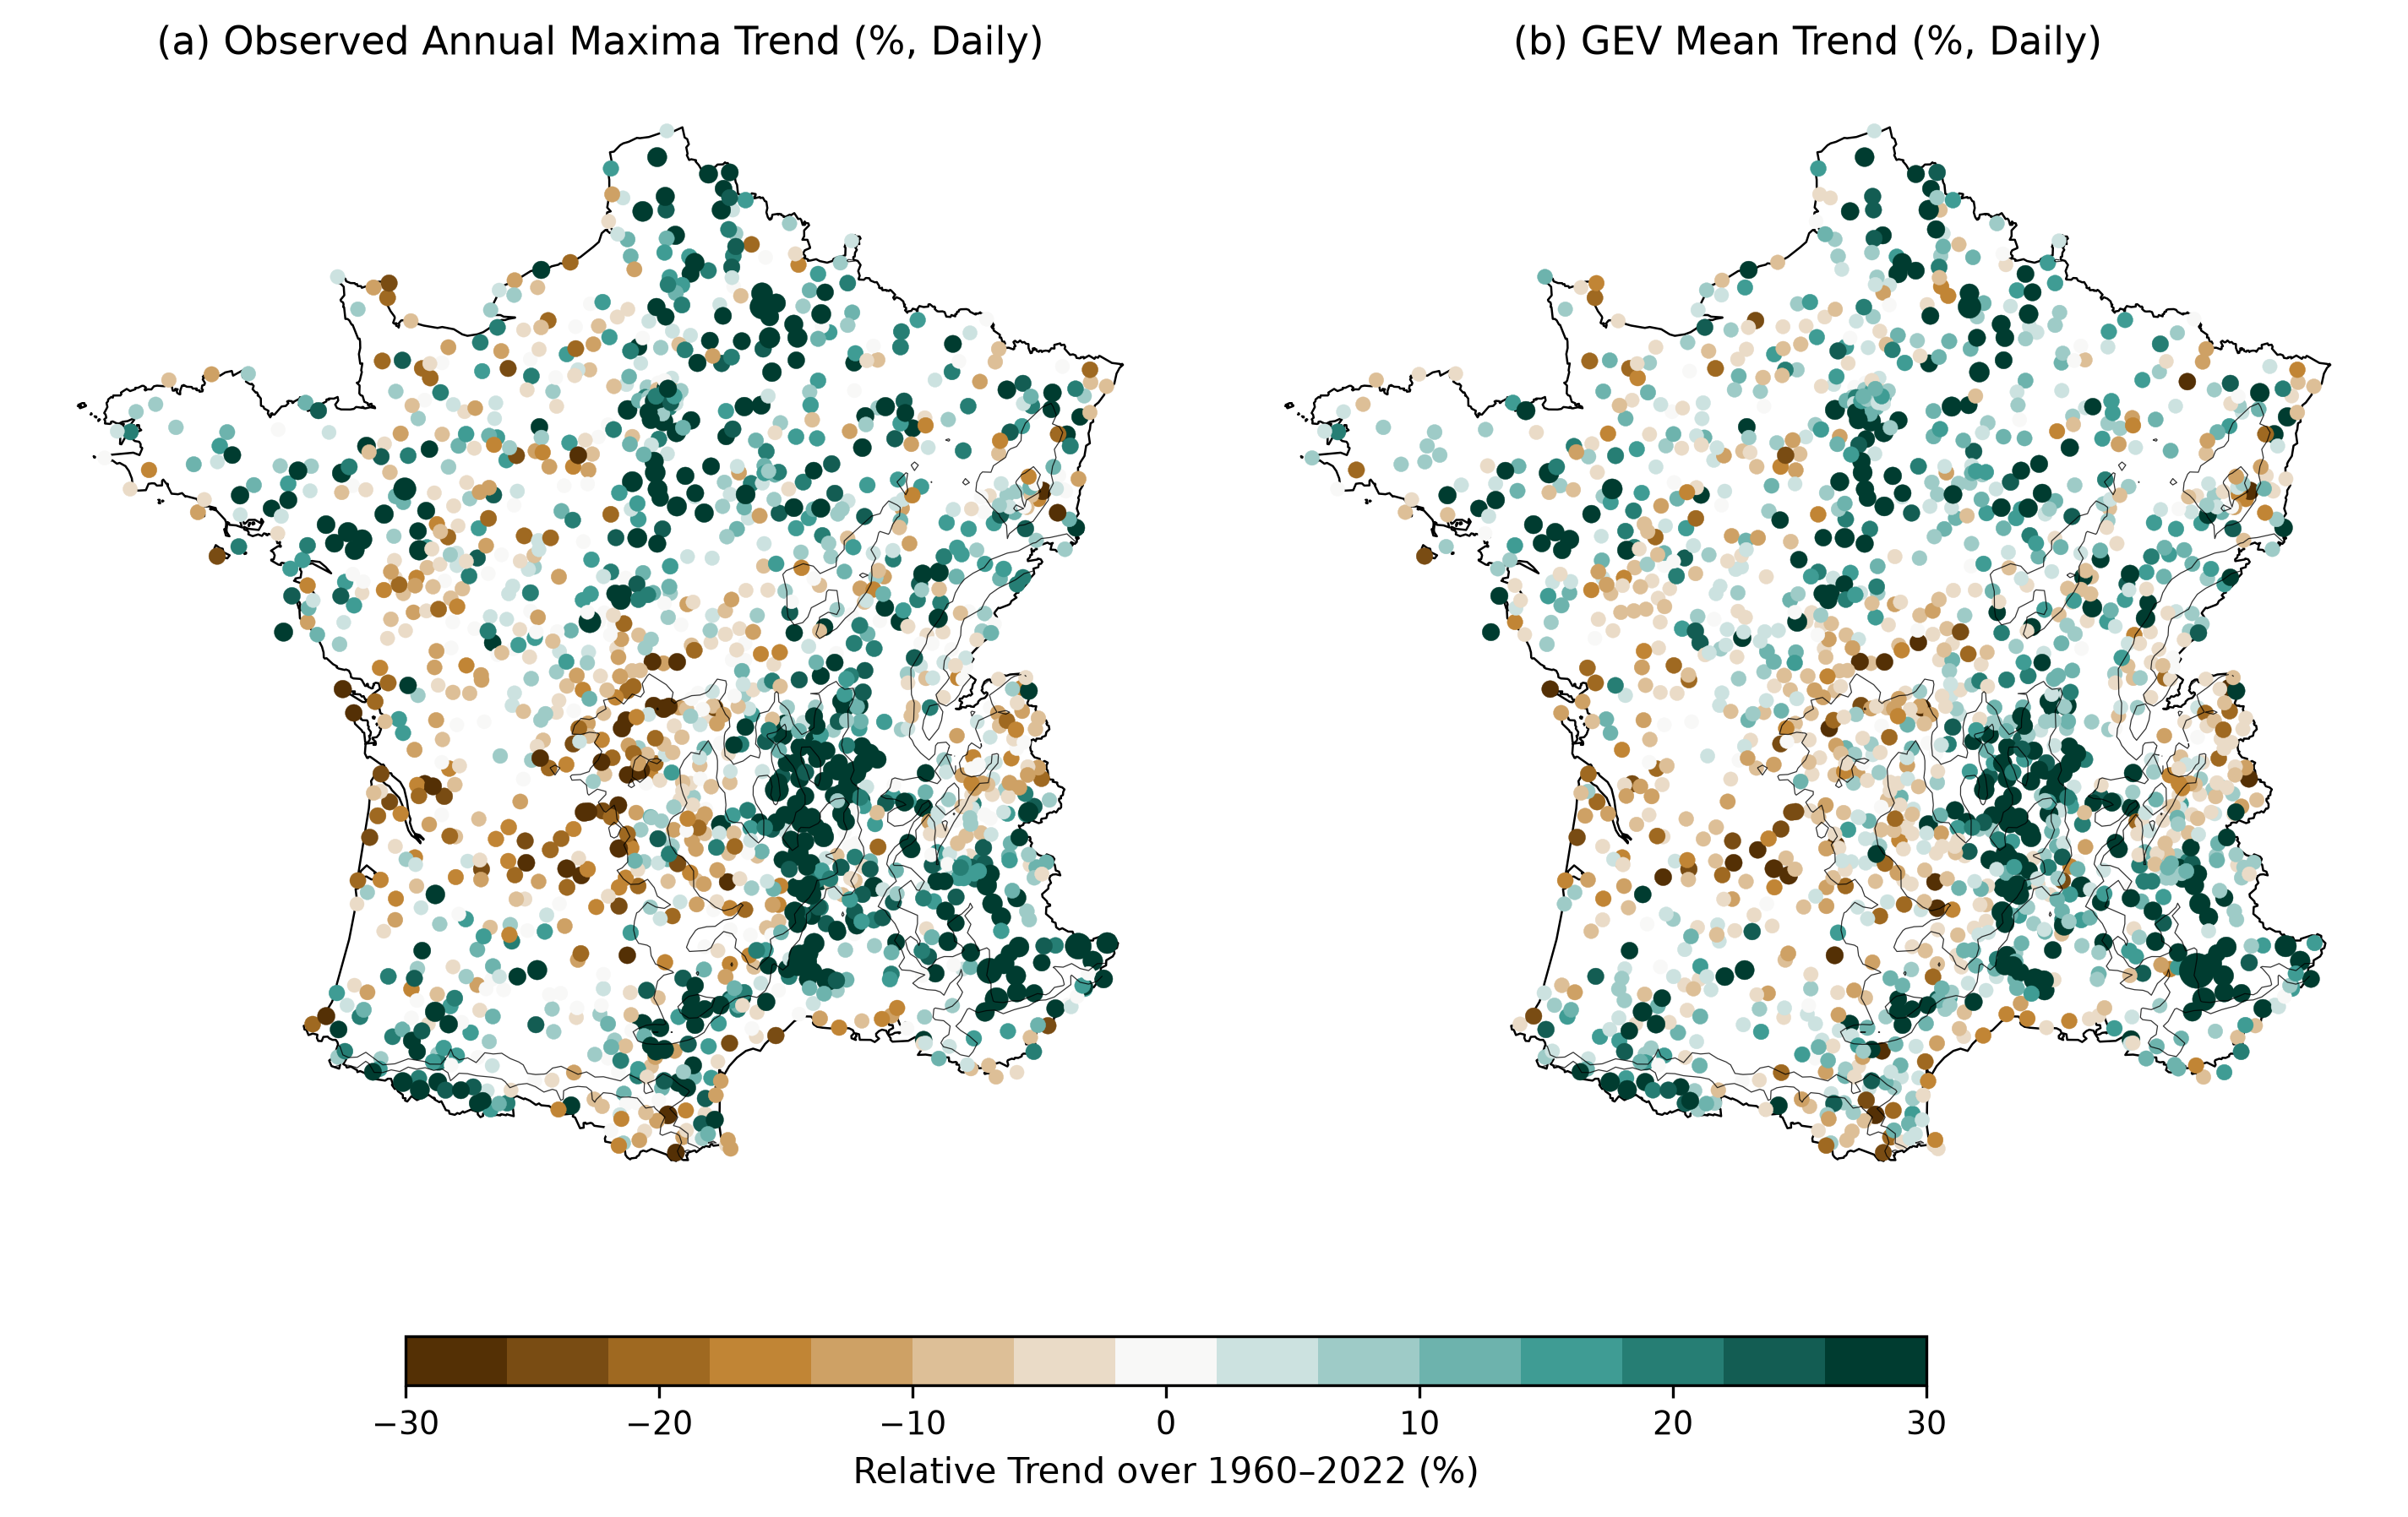
\includegraphics[width=0.62\linewidth,height=\textheight,keepaspectratio]{Figures/comparison_maxima_gev_maps_daily.png}

}

\caption{\label{fig-maxima-gev-maps-daily}\small Comparison of the
spatial distribution of relative daily trends (\%) over 1960--2022
across all 1,558 daily stations: (a) observed annual maxima trend
obtained by simple linear regression; (b) GEV-estimated mean trend.}

\end{figure}%

\begin{figure}

\centering{

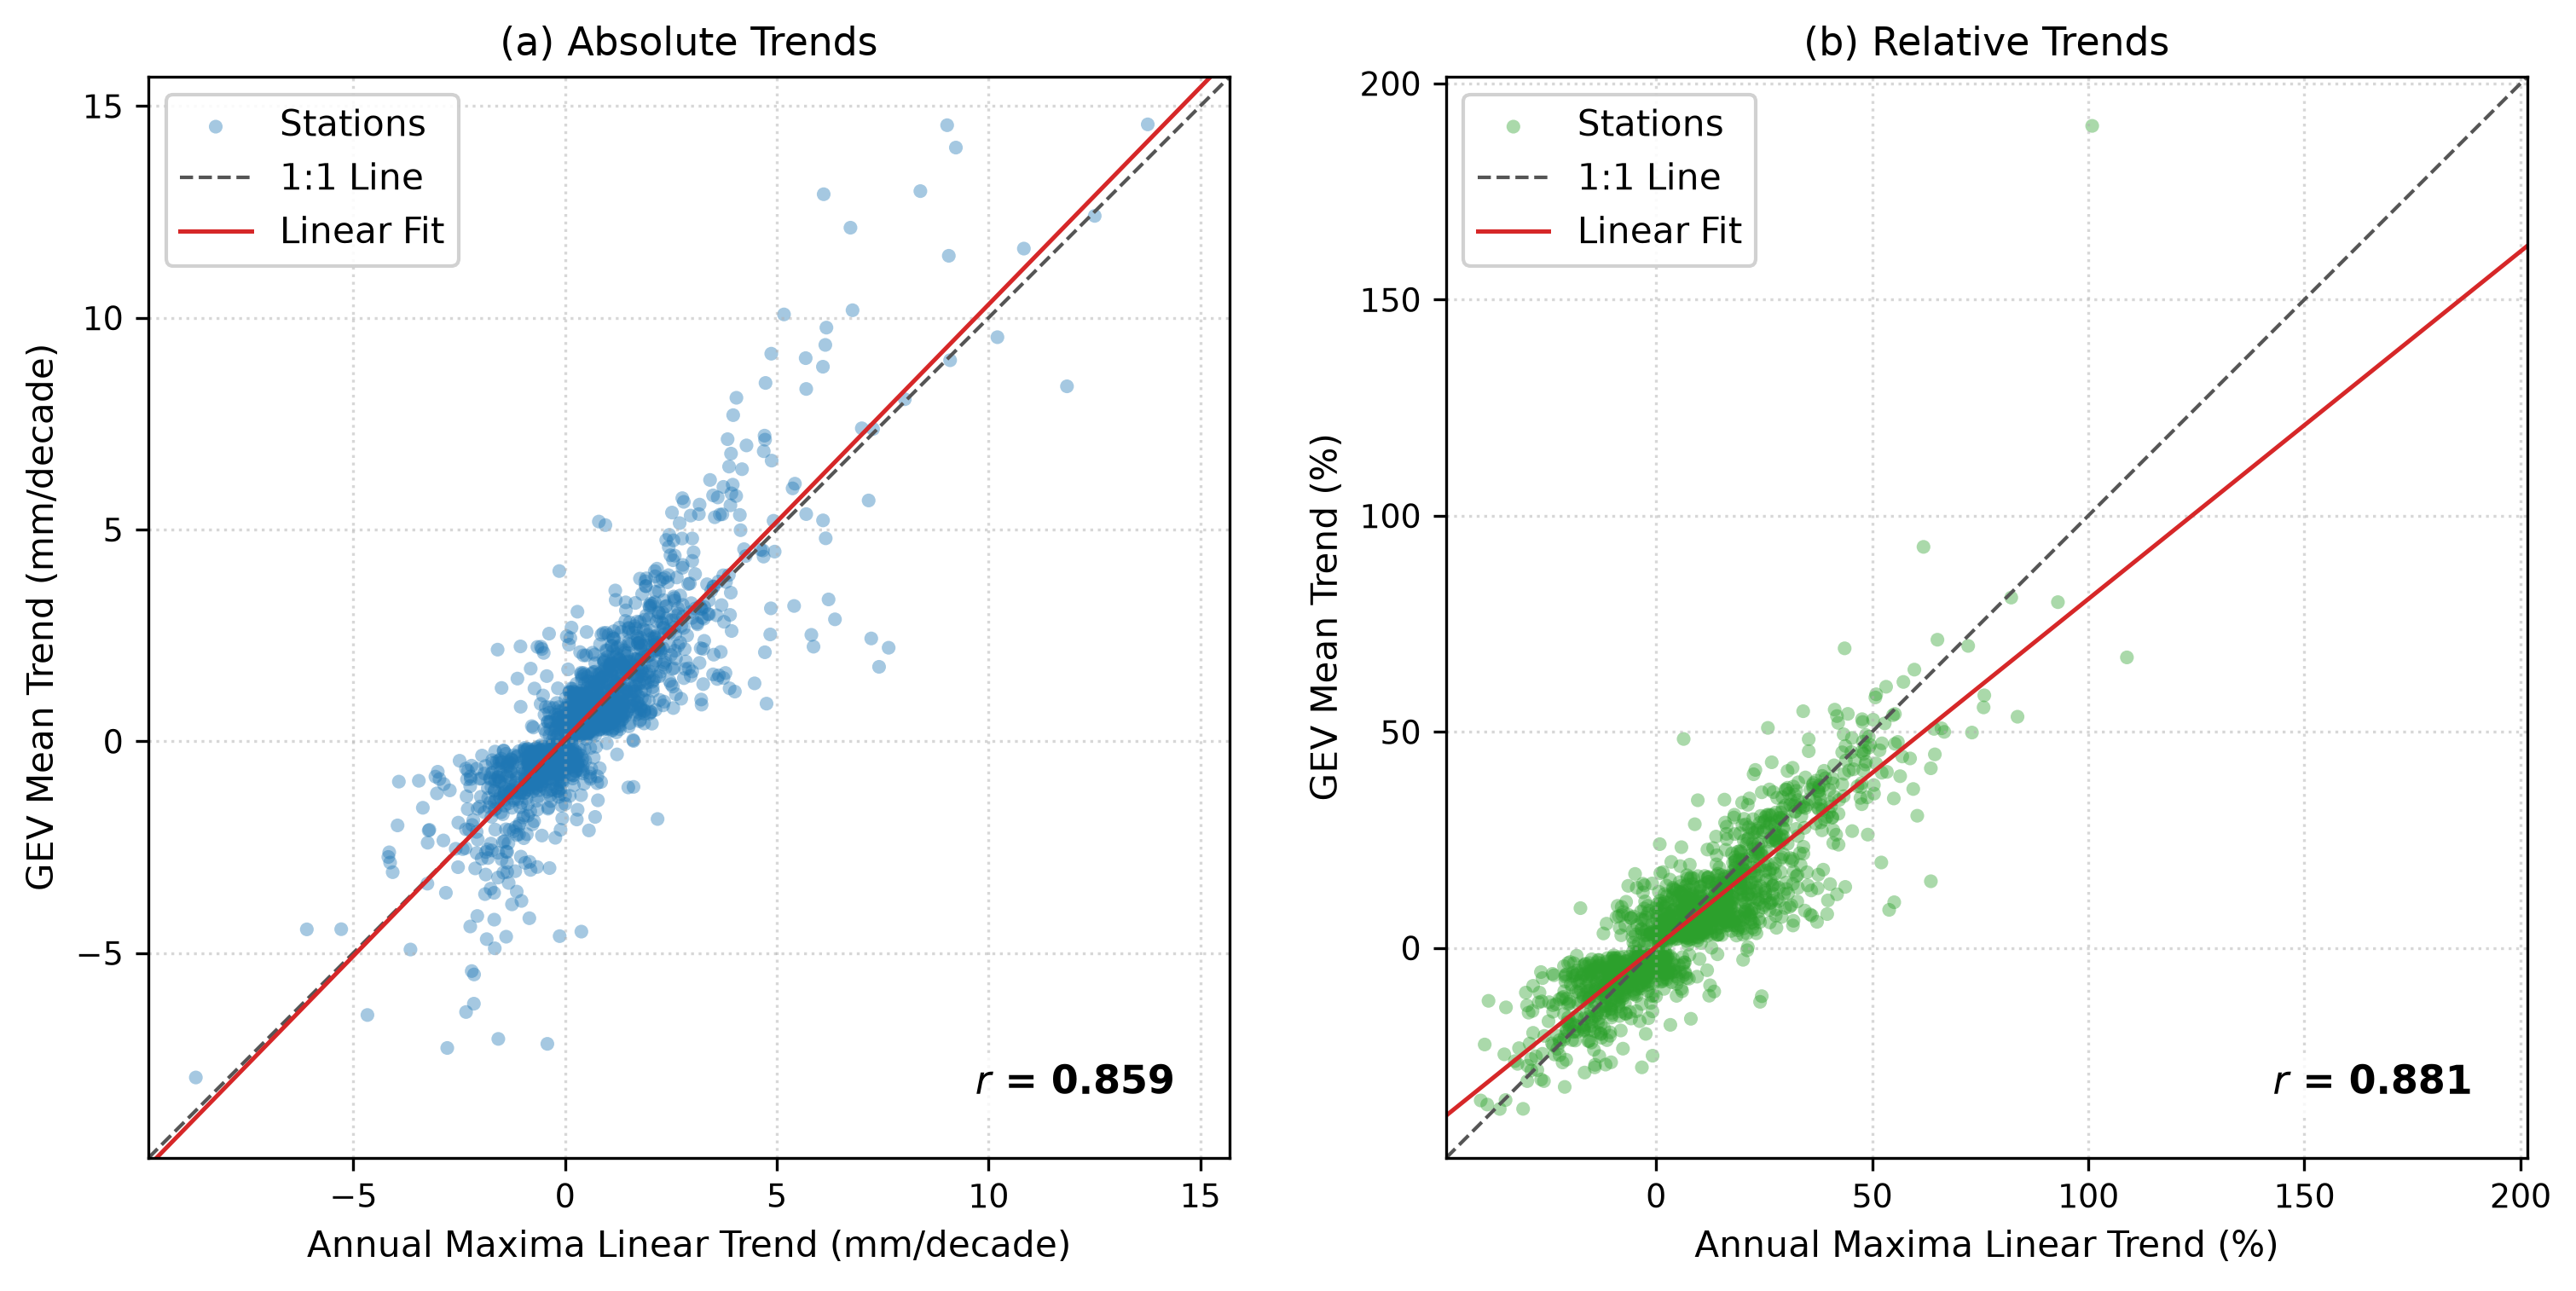
\includegraphics[width=0.6\linewidth,height=\textheight,keepaspectratio]{Figures/comparison_maxima_gev_scatter_daily.png}

}

\caption{\label{fig-maxima-gev-scatter-daily}\small Scatter plots of
GEV-estimated daily mean trend vs.~observed daily annual maxima trend
across all 1,558 daily stations: (a) absolute trends in mm/decade; (b)
relative trends in \%. The 1:1 line is shown in dashed grey, and the
linear regression fit is in red, with Pearson correlation coefficients
(\(r\)) indicated.}

\end{figure}%

\clearpage

\begin{figure}

\centering{

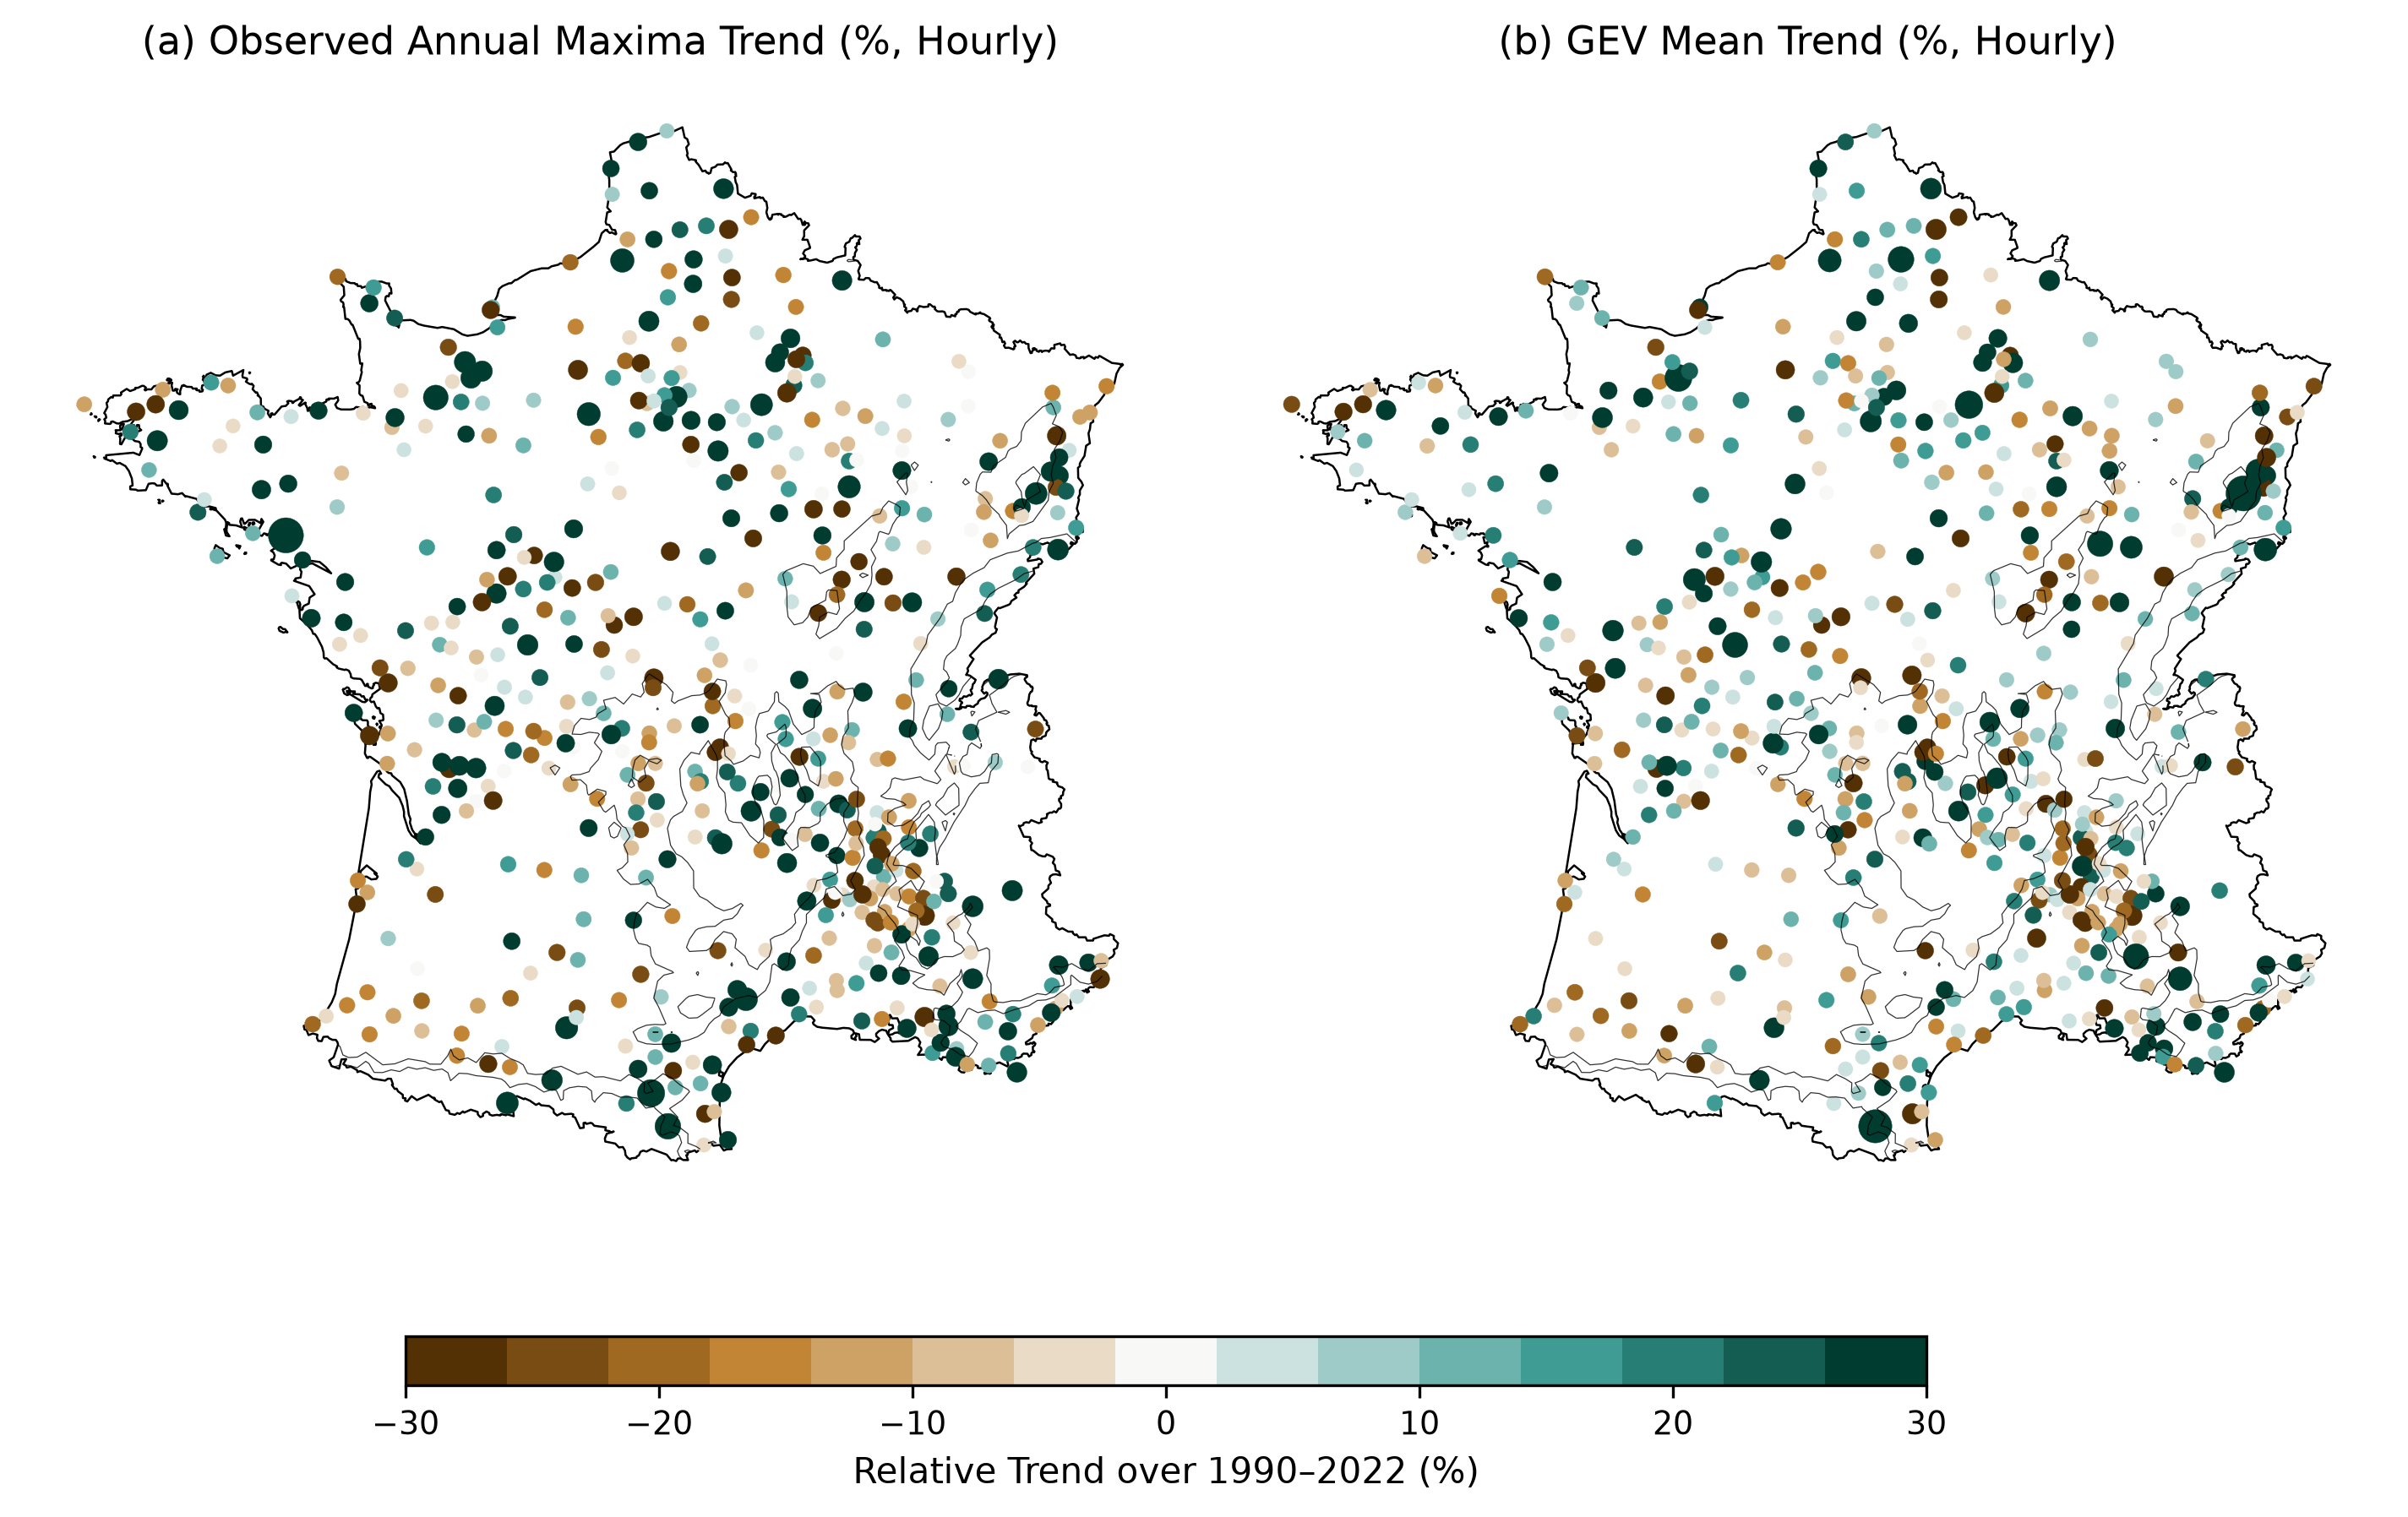
\includegraphics[width=0.62\linewidth,height=\textheight,keepaspectratio]{Figures/comparison_maxima_gev_maps_hourly.png}

}

\caption{\label{fig-maxima-gev-maps-hourly}\small Comparison of the
spatial distribution of relative hourly trends (\%) over 1990--2022
across all 562 hourly stations: (a) observed annual maxima trend
obtained by simple linear regression; (b) GEV-estimated mean trend.}

\end{figure}%

\begin{figure}

\centering{

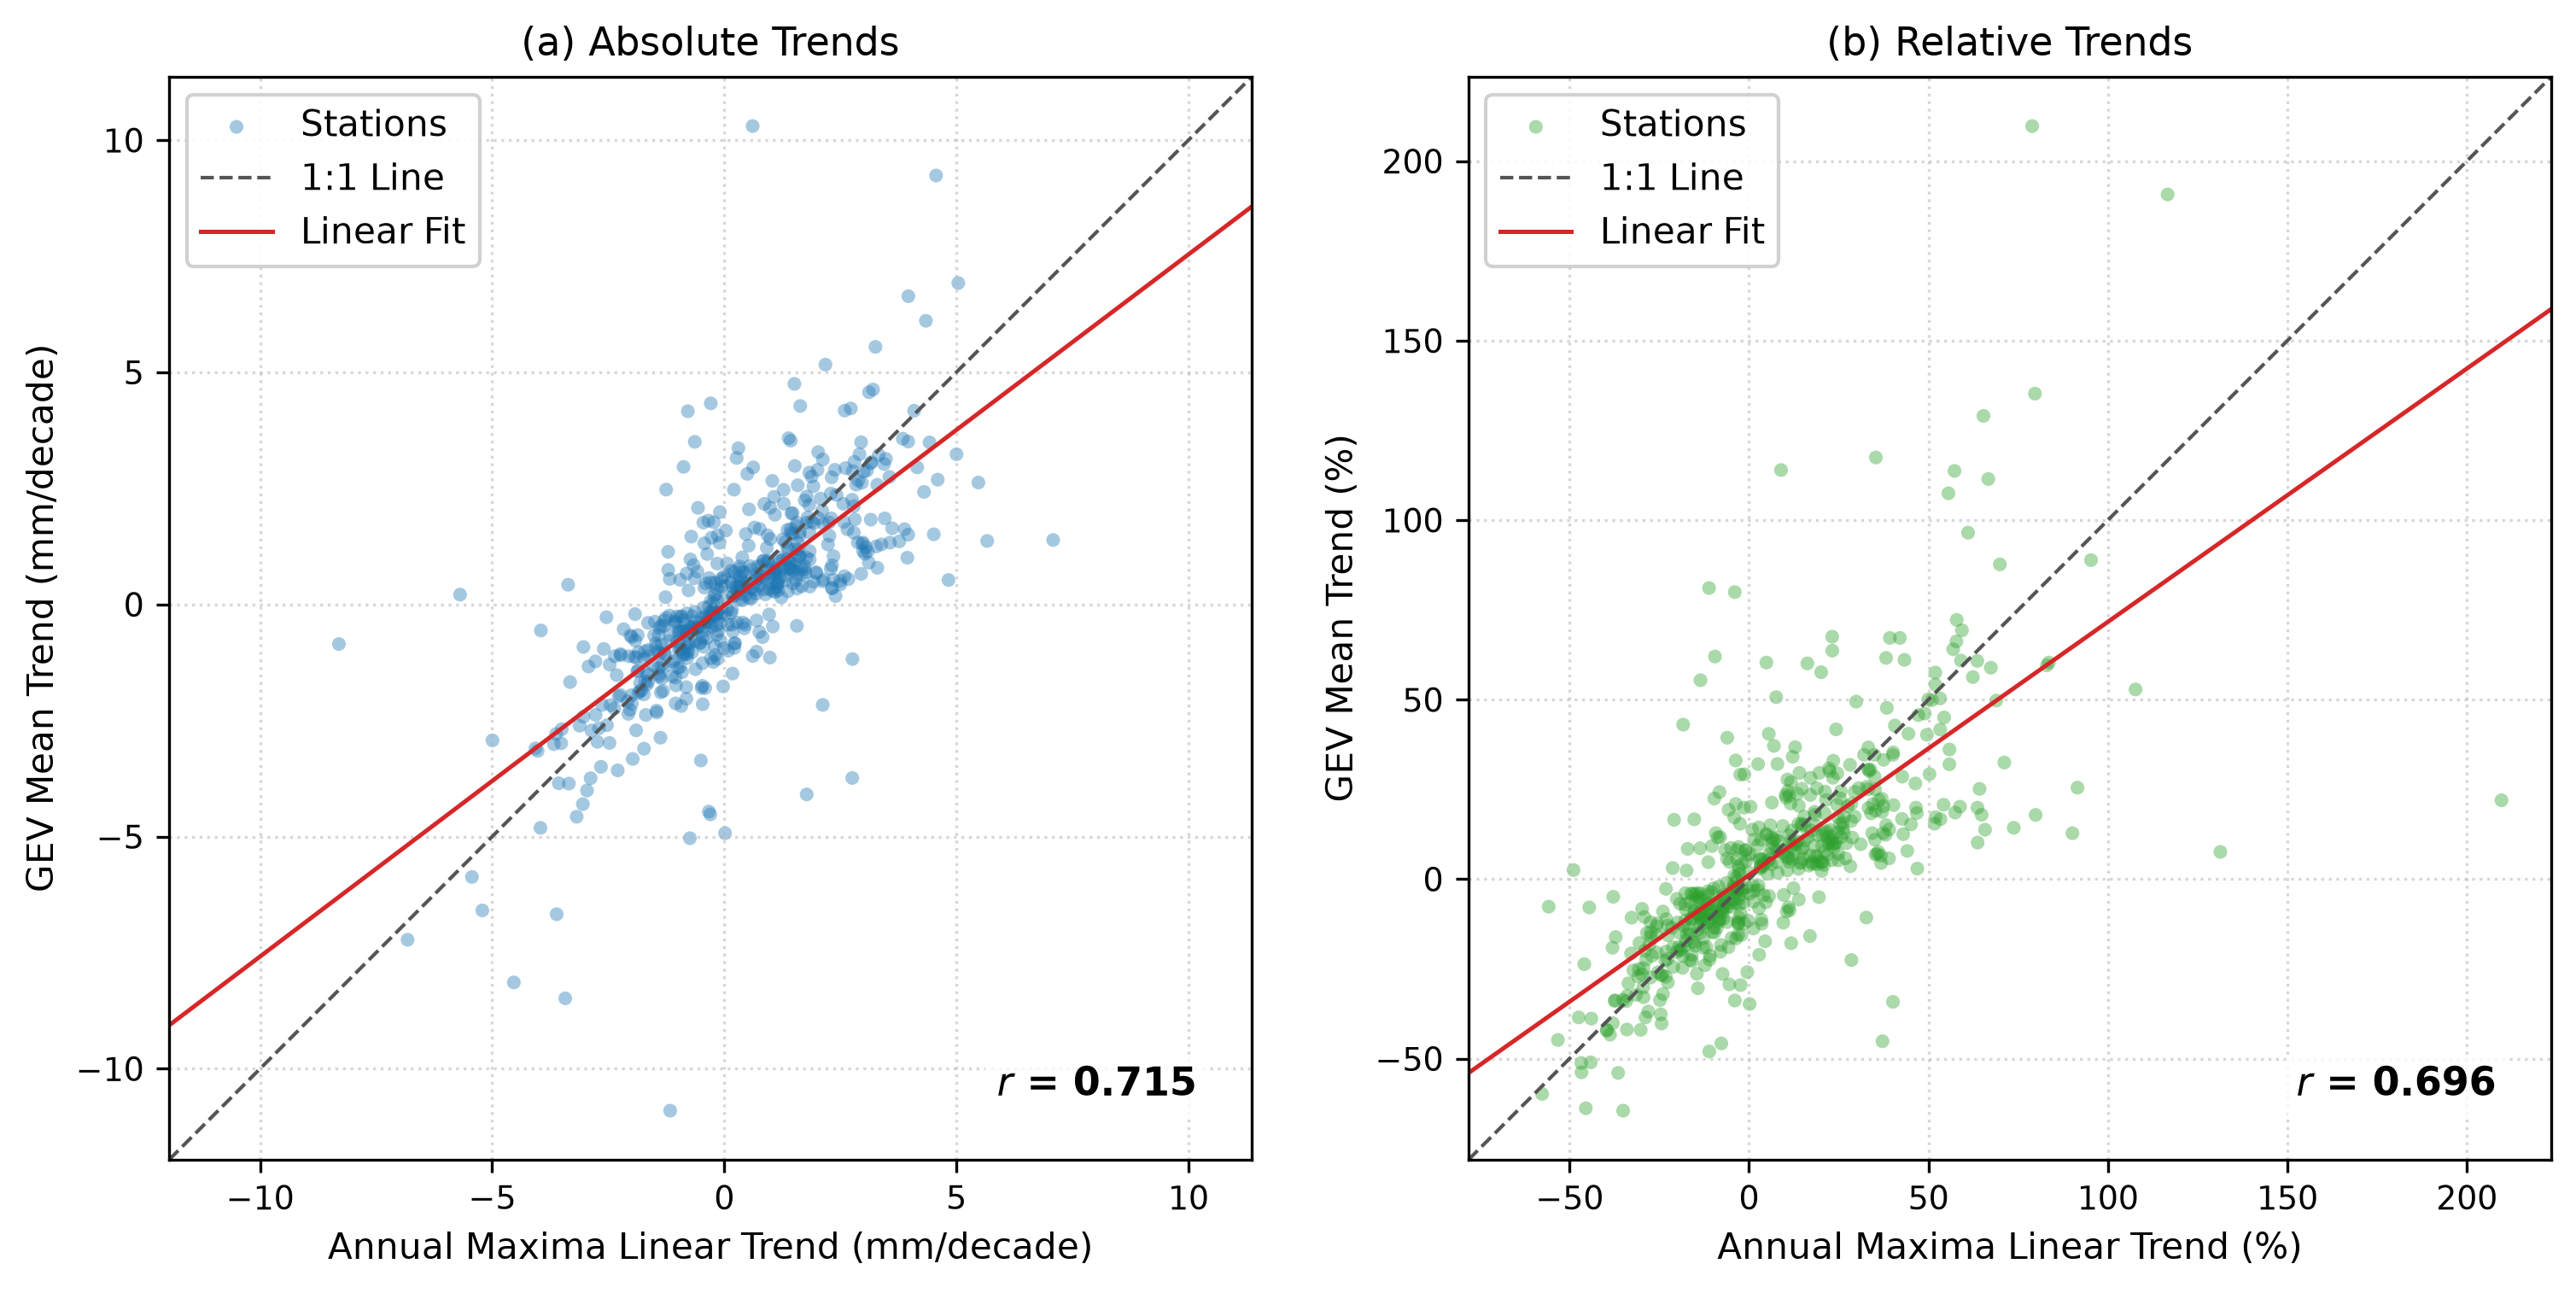
\includegraphics[width=0.6\linewidth,height=\textheight,keepaspectratio]{Figures/comparison_maxima_gev_scatter_hourly.png}

}

\caption{\label{fig-maxima-gev-scatter-hourly}\small Scatter plots of
GEV-estimated hourly mean trend vs.~observed hourly annual maxima trend
across all 562 hourly stations: (a) absolute trends in mm/decade; (b)
relative trends in \%. The 1:1 line is shown in dashed grey, and the
linear regression fit is in red, with Pearson correlation coefficients
(\(r\)) indicated.}

\end{figure}%

\clearpage

\subsection{\texorpdfstring{Comment 2: Redundancy of \(M^{*}\) Models
for Hourly
Data}{Comment 2: Redundancy of M\^{}\{*\} Models for Hourly Data}}\label{comment-2-redundancy-of-m-models-for-hourly-data}

\emph{Hourly data mostly starts in 1990. Thus, the \(M\) models are
applied just to the daily case, right? Do you really need 6
non-stationary models? In how many cases the \(M^*\) models resulted
better than the \(M\) ones?}

\begin{itemize}
\tightlist
\item
  \textbf{Response:} We appreciate this comment. Indeed, for the hourly
  case (1990-2022), because the records begin after 1985, the breakpoint
  models (\(M^{*}\)) are mathematically equivalent to the standard
  linear models (\(M\)) since all observations lie after the breakpoint
  (\(t\geq 1985\)). For the daily case (1959-2022), the \(M^{*}\) models
  represent a physical hypothesis of a trend emerging in the mid-1980s.
\end{itemize}

To address this comment, we present the table below (Response
Table~\ref{tbl-mstar-selection}) showing the full breakdown of selected
models: the stationary model (\(M_0\), representing no significant trend
at the 10\% significance level), standard linear trend models (\(M\)),
and breakpoint models (\(M^*\)). In this way, the percentages for each
subset sum to 100\%.

For the grid point percentages (AROME), the statistics are calculated
over the entire domain of mainland France. To ensure this does not
introduce spatial representation biases, we also computed these
statistics restricted only to the grid points closest to the daily
stations (\(N = 7,486\)). The results are highly consistent: for the
Annual period, selection rates at matched grid points are 75.6\% for
\(M_0\), 11.3\% for \(M\), and 13.0\% for \(M^*\) (compared to 75.5\%,
11.8\%, and 12.7\% over all mainland grid points). We therefore present
the full-grid statistics in the table to reflect the complete spatial
support of the model.

\begin{table}

\caption{\label{tbl-mstar-selection}Percentage of locations where each
model category is selected as the best fit for daily precipitation
extremes (\(M_0\) representing no trend, \(M\) a linear trend, and
\(M^*\) a breakpoint trend starting in 1985). All percentages sum to
100\% for each subset.}

\centering{

\centering
\begin{tabular}{lcccccc}
\hline
\textbf{Period} & \multicolumn{3}{c}{\textbf{Stations (Obs.)}} & \multicolumn{3}{c}{\textbf{Grid Points (AROME)}} \\
\cline{2-4} \cline{5-7}
 & \textbf{$M_0$} & \textbf{$M$} & \textbf{$M^*$} & \textbf{$M_0$} & \textbf{$M$} & \textbf{$M^*$} \\
\hline
\textbf{Annual} (YEAR) & 66.1\% & 17.8\% & 16.0\% & 75.5\% & 11.8\% & 12.7\% \\
\textbf{Autumn} (OND)  & 62.8\% & 16.2\% & 21.0\% & 73.5\% & 7.9\%  & 18.6\% \\
\textbf{Winter} (JFM)  & 64.5\% & 22.6\% & 12.9\% & 65.6\% & 22.5\% & 11.9\% \\
\textbf{Spring} (AMJ)  & 62.1\% & 16.6\% & 21.3\% & 75.0\% & 11.7\% & 13.3\% \\
\textbf{Summer} (JAS)  & 68.8\% & 14.2\% & 17.1\% & 65.6\% & 10.5\% & 24.0\% \\
\hline
\end{tabular}

}

\end{table}%

\textbf{Manuscript modifications:}

\begin{itemize}
\tightlist
\item
  In \texttt{Section\ 3.2.2\ (Model\ selection)}, we have explicitly
  clarified that the model selection procedure defaults to the standard
  linear models (\(M\)) for the hourly series.
\item
  In \texttt{Section\ 4.2.1\ (Daily)}, we have added a sentence stating
  the percentage of stations and grid points where \(M_0\), \(M\), and
  \(M^*\) models were selected.
\item
  In \texttt{Section\ 4.2.2\ (Hourly)}, we have added a sentence stating
  the percentage of stations and grid points where \(M_0\) and \(M\)
  models were selected.
\end{itemize}

\subsection{Comment 3: Rationale for the Two-Step Model
Selection}\label{comment-3-rationale-for-the-two-step-model-selection}

\emph{Not clear to me why you use the 2-step procedure, why not simply
choosing the model with the smallest p-value?}

\begin{itemize}
\tightlist
\item
  \textbf{Response:} We agree that the rationale behind this selection
  procedure should be explained more clearly. The likelihood ratio test
  compares each non-stationary model \(M_{j}\) (\(j\geq 1\)) to the
  stationary model \(M_{0}\). However, models \(M_{3}\) and
  \(M_{3}^{*}\) (where both \(\mu\) and \(\sigma\) vary over time) have
  2 degrees of freedom more than \(M_{0}\), whereas models
  \(M_{1}/M_{1}^{*}\) and \(M_{2}/M_{2}^{*}\) have only 1 degree of
  freedom more. Choosing the model with the absolute smallest p-value
  across different degrees of freedom can bias the selection toward
  simpler and thus more constrained models. Our 2-step procedure is
  designed to first test if a trend in both location and scale
  (\(M_{3}\) or \(M_{3}^{*}\)) is statistically justified. If it is not,
  we look at whether a simpler trend in either location only
  (\(M_{1}/M_{1}^{*}\)) or scale only (\(M_{2}/M_{2}^{*}\)) is
  justified. This favors more flexible models (i.e.~both parameters
  changing) when statistically supported.
\end{itemize}

\textbf{Manuscript modifications:}

\begin{itemize}
\tightlist
\item
  In \texttt{Section\ 3.2.2\ (Model\ selection)}, we have added the
  following clarifications: ``\emph{We apply for each non-stationary
  model \(M_{j}\), \(j \ge 1\), a likelihood ratio test to compare the
  goodness of fit of \(M_{j}\) to that of the stationary model
  \(M_{0}\), accounting for their respective number of parameters to
  avoid overfitting {[}\ldots{]} This two-step process prioritizes
  models with simultaneous temporal effects on \(\mu\) and \(\sigma\)
  when statistically justified, ensuring complexity is introduced only
  when it provides plus-value.}''
\end{itemize}

\subsection{Comment 4: Clarification of Evaluation
Metrics}\label{comment-4-clarification-of-evaluation-metrics}

\emph{I suggest to illustrate in the method section which evaluation
metrics you used (e.g.~ME, r) and for which variables other than 10-yr
RL (e.g.~frequency of wet days)}

\begin{itemize}
\tightlist
\item
  \textbf{Response:} We agree. The subsection defining the agreement
  metrics (Pearson correlation \(r\), Mean Error \(ME\), and relative
  bias in \%) and introducing all the evaluated variables (mean number
  of wet days, mean annual total precipitation, daily and hourly 10-year
  return levels) was indeed lacking in the first version of this
  article.
\end{itemize}

\textbf{Manuscript modifications:}

\begin{itemize}
\tightlist
\item
  In the revised manuscript, we have added an new
  \texttt{Section\ 3.3\ (Assessing\ the\ agreement\ between\ AROME\ and\ the\ stations)}:
\end{itemize}

\begin{quote}
\subsection{Assessing the agreement between AROME and the stations}\label{assessing}

To evaluate the CNRM-AROME model against observations, each Météo-France
station is matched to the closest model grid point (2.5 km \(\times\)
2.5 km) based on its geographic location. This pairing allows assessing
the spatial and temporal coherence of simulated fields against raingauge
measurements.

We assess the model's agreement using three main metrics:

\begin{enumerate}
    \item \textbf{Pearson correlation coefficient ($r$):} Used to quantify the spatial consistency between observed and simulated fields across all station locations.
    \item \textbf{Mean Error ($ME$, or absolute bias):} Measures the average difference between the simulated and observed statistics, defined as:
    \begin{equation}
        ME = \frac{1}{n}\sum_{i=1}^{n} (Y_{i,\text{AROME}} - Y_{i,\text{OBS}})
    \end{equation}
    where $Y_i$ represents the climatological or trend statistic computed at station $i$ (or its closest model grid point) and $n$ is the total number of compared stations.
    \item \textbf{Relative Bias ($RB$, \%):} Expresses the bias as a percentage of the observed baseline, which is particularly useful for comparing regions with highly contrasted precipitation baselines:
    \begin{equation}
        RB = 100 \times \frac{\sum_{i=1}^{n} (Y_{i,\text{AROME}} - Y_{i,\text{OBS}})}{\sum_{i=1}^{n} Y_{i,\text{OBS}}} = 100 \times \frac{ME}{\bar{Y}_{\text{OBS}}}
    \end{equation}
    where $\bar{Y}_{\text{OBS}}$ is the mean of the observed values across all compared stations.
\end{enumerate}

These metrics are calculated for five core precipitation indices: the
annual frequency of wet days (daily precipitation exceeding 1,mm), the
mean annual total precipitation, the daily and hourly 10-year return
levels, and the relative trends in daily and hourly 10-year return
levels. Climatological indices are evaluated in a stationary framework,
whereas relative trends are obtained from the estimated non-stationary
GEV distributions (cf.~Section 3.2.1). In the latter case, we do not
compute the relative bias as relative trends are already \%.
\end{quote}

\subsection{Comment 5: Introduction of Relative
Biases}\label{comment-5-introduction-of-relative-biases}

\emph{I strongly suggest to add information on relative biases (also, in
figures 4 and 5), because N mm/year could be small or big difference
depending on the baseline!}

\begin{itemize}
\tightlist
\item
  \textbf{Response:} We agree with the reviewer. Relative biases
  (expressed in \%) are more informative for comparing regions with
  highly contrasted precipitation baselines, such as the dry
  Mediterranean coastal areas and wet mountainous regions.
\end{itemize}

\textbf{Manuscript modifications:}

\begin{itemize}
\tightlist
\item
  In
  \texttt{Section\ 3.3\ (Assessing\ the\ agreement\ between\ AROME\ and\ the\ stations)},
  we have defined the Relative Bias (\(RB\), \%) metric to quantify
  systematic errors relative to the observed baselines.
\item
  In
  \texttt{Section\ 4.1\ (Evaluation\ of\ the\ precipitation\ climatology\ of\ AROME)},
  the climatology maps (Figure 3) have been updated to add the relative
  bias (in \%) in the fourth row, and the caption has been updated
  accordingly.
\item
  In the same section, we have added a second panel to Figure 4 showing
  the seasonal evolution of the relative bias (in \%) for the four
  climatological indices.
\end{itemize}

\subsection{Comment 6: Presentation of Bias at the Hourly
Scale}\label{comment-6-presentation-of-bias-at-the-hourly-scale}

\emph{This seems mostly referring to spatial correlation; but also bias
should be mentioned (e.g., underestimation at 1h)}

\begin{itemize}
\tightlist
\item
  \textbf{Response:} We have revised this paragraph to explicitly
  mention the seasonal variations in bias, in addition to the spatial
  correlation. Specifically, we have highlighted the systematic
  underestimation of hourly extremes (1h 10-year return level) by AROME,
  which is particularly pronounced during the convective seasons (spring
  and summer).
\end{itemize}

\textbf{Manuscript modifications:}

\begin{itemize}
\item
  At the end of
  \texttt{Section\ 4.1\ (Evaluation\ of\ the\ precipitation\ climatology\ of\ AROME)},
  the summary paragraph has been revised to explicitly mention the
  systematic underestimation of hourly extremes alongside the lower
  spatial agreement in spring:

  \begin{quote}
  \emph{``In summary, AROME shows a good representation of the
  climatology of precipitation extremes that encourages us to continue
  evaluation on trends, keeping however in mind that hourly extremes are
  systematically underestimated by the model throughout the year
  (especially during spring and summer) and exhibit a lower spatial
  agreement in spring.''}
  \end{quote}
\end{itemize}

\subsection{Comment 7: Climatology Maps Customization (Figure
3)}\label{comment-7-climatology-maps-customization-figure-3}

\emph{I suggest to substitute 3rd row or add a 4th row with relative
biases. For all figures with maps: Use same size for dots (now, the
highest values have both darker color and bigger size, hiding other; I
think color is enough); maybe find a darker color for the 0 bios (not
much visible as it is now).}

\begin{itemize}
\tightlist
\item
  \textbf{Response:} We thank the reviewer for these suggestions, which
  significantly improve the readability of the maps.
\end{itemize}

\textbf{Manuscript modifications:}

\begin{enumerate}
\def\labelenumi{\arabic{enumi}.}
\item
  In
  \texttt{Section\ 4.1\ (Evaluation\ of\ the\ precipitation\ climatology\ of\ AROME)},
  we have added a fourth row to the climatology maps (Figure 3) to
  present the relative bias (\%) alongside the absolute difference in
  the third row, making the regional comparisons clearer while
  preserving the absolute magnitude information.
\item
  In all map figures across the manuscript (Figure 3 in
  \texttt{Section\ 4.1}, Figures 5 and 6 in
  \texttt{Sections\ 4.2}/\texttt{4.3}, and the monthly trend maps in
  \texttt{Appendix\ C}), we have used a uniform dot size for all
  displayed stations so that larger dots do not obscure adjacent
  stations.
\item
  In
  \texttt{Section\ 4.1\ (Evaluation\ of\ the\ precipitation\ climatology\ of\ AROME)},
  the color scale of the climatology maps (Figure 3) has been modified
  so that a zero bias is represented by a clearly visible grey fill.
\item
  In the trend maps of
  \texttt{Section\ 4.2\ (Spatial\ distribution\ of\ precipitation\ trends)},
  \texttt{Section\ 4.3\ (Seasonal\ variations\ of\ hourly\ trends)}, and
  the monthly maps in \texttt{Appendix\ C}, we adopted the following
  display conventions for station markers and grid cell masks:
\end{enumerate}

\begin{longtable}[]{@{}
  >{\raggedright\arraybackslash}p{(\linewidth - 2\tabcolsep) * \real{0.4000}}
  >{\raggedright\arraybackslash}p{(\linewidth - 2\tabcolsep) * \real{0.6000}}@{}}
\toprule\noalign{}
\begin{minipage}[b]{\linewidth}\raggedright
Type
\end{minipage} & \begin{minipage}[b]{\linewidth}\raggedright
Display
\end{minipage} \\
\midrule\noalign{}
\endhead
\bottomrule\noalign{}
\endlastfoot
\textbf{Non-significant} (stations) & Open circle: white fill, light
grey outline \\
\textbf{Significant ≈ 0} (stations) & Filled grey disk, dark outline \\
\textbf{Significant coloured} (stations) & Trend colour on the map
scale; \textbf{uniform marker size} \\
\textbf{AROME grid} & Non-significant grid points \textbf{not
displayed} \\
\end{longtable}

\subsection{Comment 8: Seasonal Bias Synthesis (Figure
4)}\label{comment-8-seasonal-bias-synthesis-figure-4}

\emph{I suggest a second panel summarizing \%biases for the 4
variables.}

\begin{itemize}
\tightlist
\item
  \textbf{Response:} We agree. We have added a second panel to the
  seasonal synthesis figure showing the seasonal evolution of the
  relative bias (\%) for the four precipitation indices. This provides a
  concise and complete seasonal comparison of both spatial correlation
  and bias.
\end{itemize}

\textbf{Manuscript modifications:}

\begin{itemize}
\tightlist
\item
  In
  \texttt{Section\ 4.1\ (Evaluation\ of\ the\ precipitation\ climatology\ of\ AROME)},
  Figure 4 (seasonal synthesis) has been updated to include a second
  panel (b) presenting the seasonal relative bias (in \%) for the four
  precipitation indices, and the caption has been updated to describe
  both panels.
\end{itemize}


\includegraphics[width=1\linewidth,height=\textheight,keepaspectratio]{./final/fig4.pdf}
\emph{\emph{Article Figure 4.} Seasonal synthesis of the climatological
agreement between the AROME model and Météo-France stations for the four
precipitation indices: (a) spatial Pearson correlation (\(r\)) and (b)
relative bias (\(RB\), in \%) depending on the season.}

\subsection{Comment 9: Restructuring the Monthly Trend Mapping (Figure 8
\&
9)}\label{comment-9-restructuring-the-monthly-trend-mapping-figure-8-9}

\emph{I found this text a too qualitative, and all those maps in figure
8 not much relevant and their metrics not easily readable. My suggestion
is to move this figure in supplementary, and to update figure 9 to give
more complete summary information about monthly performance (not just
r): trend from stations and model, bias, correlation for both daily and
hourly extremes (example or organization below, or any other combination
allowing to show all those metrics). It could support what you then
mention at line 377 in the discussion.}

\begin{itemize}
\tightlist
\item
  \textbf{Response:} We agree with this suggestion. The monthly maps of
  hourly trends are dense and difficult to read.
\end{itemize}

\begin{enumerate}
\def\labelenumi{\arabic{enumi}.}
\item
  We have moved the monthly trend maps to the Appendix.
\item
  We have redesigned the summary figure (Figure 7) as a three-panel
  bar-chart synthesis for both daily (1959--2022) and hourly
  (1990--2022) extremes: \textbf{(a)} monthly median GEV relative
  trends, with side-by-side subpanels for Météo-France stations and
  AROME; \textbf{(b)} monthly mean error (ME, \%) in relative trends
  between AROME and stations; and \textbf{(c)} monthly spatial
  correlation (\(r\)) of GEV relative trends. This structured summary
  makes the monthly analysis much more quantitative and readable.
\end{enumerate}

\textbf{Manuscript modifications:}

\begin{itemize}
\item
  In \texttt{Section\ 4.2.2\ (Hourly)}, the maps of monthly trends
  (formerly Figure 8) have been moved to Appendix C as Figure C1.
\item
  In \texttt{Section\ 4.2.2\ (Hourly)}, the section describing monthly
  trends has been rewritten to be more quantitative, referencing the new
  Figure 8 to detail the median trends, relative biases, and spatial
  correlations:

  \begin{quote}
  \textbf{Section 4.2.2 (Monthly refinement):} ``The monthly analysis
  (Figure 7) further highlights the specificity of convective regimes
  and the strong temporal concentration of some signals. Figure 7a
  compares the monthly median GEV relative trends at Météo-France
  stations and the corresponding AROME grid points (side-by-side
  subpanels). At the daily scale, station median trends remain moderate
  throughout the year, ranging from \(-16.27\%\) in September to
  \(+14.05\%\) in April/May. In contrast, station-based hourly GEV
  trends show far larger values concentrated in specific convective
  windows, with monthly medians reaching \(+43.28\%\) in February,
  \(+28.26\%\) in March, \(+101.86\%\) in June, \(+53.88\%\) in October,
  and \(+30.09\%\) in December. AROME reproduces the positive sign of
  these monthly trend peaks but systematically underestimates their
  magnitude. For instance, in June, AROME simulates a median hourly GEV
  trend of \(+17.70\%\) (against \(+101.86\%\) for stations), and in
  February, it simulates \(+11.46\%\) (against \(+43.28\%\) for
  stations).

  This systematic underestimation is reflected in the monthly mean
  errors (\(ME\)) between the corresponding AROME grid points and
  stations shown in Figure 7b, with large negative values at the hourly
  scale during convective months (e.g., \(ME = -75.6\%\) in February,
  \(ME = -182.0\%\) in March, and \(ME = -136.1\%\) in June), whereas
  daily mean errors remain much smaller (e.g., \(ME = -0.9\%\) in
  January and \(ME = 3.1\%\) in March).

  Finally, Figure 7c shows that spatial correlation (\(r\)) is
  consistently higher at the daily scale (peaking at \(r = 0.62\) in
  December) than at the hourly scale. At the hourly scale, spatial
  correlations are extremely low or close to zero during the convective
  months (e.g., \(r = 0.08\) in June, \(r = 0.07\) in October,
  \(r = 0.04\) in March, and \(r = 0.02\) in May), and virtually zero in
  July and September (\(r \approx 0.00\)), reflecting the high local
  spatial variability of hourly trends. February stands out as the only
  month showing moderate spatial agreement (\(r = 0.45\)).''
  \end{quote}
\item
  The discussion section in \texttt{Section\ 5.3.2} (discussing the
  comparison of hourly signals) has been updated to refer to the new
  Figure 7 and include the quantitative statistics:

  \begin{quote}
  \textbf{Section 5.3.2:} ``AROME reproduces part of the seasonal
  structure of these hourly signals---concurring on the months
  associated with enhanced extreme activity (Figure 7a)---but fails to
  capture their spatial organization and magnitude. Figure 7a and 7b
  show that the model systematically underestimates the magnitude of
  positive hourly GEV trends, leading to a much larger underestimation
  of relative trends at hourly than at daily scale (e.g.,
  \(ME = -136.1\%\) vs.~\(-1.4\%\) in June, see Fig. 7a,b). Furthermore,
  hourly spatial correlations shown in Figure 7c remain close to zero
  for most convective months (e.g., \(r = 0.08\) in June, \(r = 0.04\)
  in March), reflecting shifts in the simulated convective precipitation
  zones, especially in mountain regions (such as the Massif Central and
  the Alps) where summer convective activity dominates. Part of this
  trend magnitude underestimation is consistent with the underestimation
  of temperature trends in AROME (Figure 8).''
  \end{quote}
\end{itemize}

\clearpage


\includegraphics[width=1\linewidth,height=\textheight,keepaspectratio]{./final/fig7.pdf}
\emph{\emph{Article Figure 7.} Monthly GEV relative trend synthesis for
both daily (1959--2022) and hourly (1990--2022) scales, calculated only
over locations with statistically significant trends at the stations (at
the 10\% level): \textbf{(a)} median GEV relative trend (\%) at
Météo-France stations (left) and corresponding AROME grid points
(right); \textbf{(b)} mean error (\(ME\), in \%) between the
corresponding AROME grid points and Météo-France stations; and
\textbf{(c)} spatial correlation (\(r\)) of GEV relative trends. Values
above each bar in panel (c) indicate the number of significant stations
used in the calculations. All statistics are evaluated at AROME grid
points corresponding to these stations. }

\clearpage

\subsubsection{Comment 10: Rain Gauge Undercatch and
Inhomogeneities}\label{comment-10-rain-gauge-undercatch-and-inhomogeneities}

\emph{Link this to your results. Should we expect even higher
underestimation at hourly scale by the model, if undercatch errors for
stations will be corrected? What do you mean with ``heterogeneity''?}

\begin{itemize}
\tightlist
\item
  \textbf{Response:} We agree. We have added a discussion linking the
  rain gauge undercatch to the model underestimation, showing that
  correcting for undercatch would likely mean that the model's
  underestimation of hourly extremes is even larger than reported. We
  have also replaced the term ``heterogeneity'' with ``inhomogeneities''
  and clarified its meaning (non-climatic shifts) and potential impact.
\end{itemize}

\textbf{Manuscript modifications:}

\begin{itemize}
\item
  In \texttt{Section\ 5.1.2\ (Limitations\ of\ the\ study)}, the
  paragraph discussing rain gauge limitations has been updated as
  follows:

  \begin{quote}
  ``First, station precipitation measurements are frequently affected by
  undercatch errors, which are particularly pronounced in cold and
  mountainous regions with strong winds. Because undercatch typically
  leads to an underestimation of actual precipitation (especially for
  high-intensity, short-duration convective events), correcting for
  these errors would increase the observed extreme values. Consequently,
  the model's underestimation of hourly extremes is likely even larger
  than what we report here. Furthermore, station time series can also
  exhibit some inhomogeneities (non-climatic shifts in the time series
  caused by changes in station location, environment, or sensor types
  over decades), which could introduce local artificial trend
  components, although the data used here have been quality-controlled
  by Météo-France.''
  \end{quote}
\end{itemize}

\subsubsection{Comment 11: Introduction of the SMEV
Approach}\label{comment-11-introduction-of-the-smev-approach}

\emph{I think SMEV approach should also be mentioned (Marra et al.~2020
10.1029/2020gl090209) which has been also applied in both stationary
mode for evaluation of short-run CPMs (Correa-Sanchez et al., 2025
\url{https://doi.org/10.1016/j.jhydrol.2025.133324}) and non-stationary
mode on 90-yr CPM (Lompi et al., 2025
\url{https://doi.org/10.1016/j.adwatres.2025.105071})}

\begin{itemize}
\tightlist
\item
  \textbf{Response:} We thank the reviewer for pointing out these highly
  relevant references. We agree that the Simplified Metastasis Extreme
  Value (SMEV) distribution is a very valuable alternative to the GEV
  for short records and sub-daily extremes. We have added a mention of
  the SMEV distribution in the limitations section, citing the three
  recommended papers.
\end{itemize}

\textbf{Manuscript modifications:}

\begin{itemize}
\item
  In \texttt{Section\ 5.1\ (Limitations\ of\ the\ study)}, the paragraph
  discussing alternative extreme value approaches has been updated as
  follows:

  \begin{quote}
  ``To make the estimation more robust, other solutions include taking
  into account threshold exceedances within a generalized Pareto
  distribution (GPD) framework, or using a distribution modeling all
  precipitation values, such as the recent extended generalized Pareto
  distribution (Haruna et al., 2025) or the Simplified Metastasis
  Extreme Value (SMEV) distribution (Marra et al., 2020; Correa-Sanchez
  et al., 2025; Lompi et al., 2025), or using a neighborhood or
  region-of-influence approach (Blanchet et al., 2021) to reduce
  sampling bias by using more data.''
  \end{quote}
\end{itemize}

\subsubsection{Minor Comments}\label{minor-comments}

\begin{itemize}
\tightlist
\item
  \textbf{Line 11 (and 395). ``added value'' \ldots{} with respect to
  what?}

  \begin{itemize}
  \tightlist
  \item
    \textbf{Response:} We agree. We have clarified that the ``added
    value'' is relative to traditional, coarser-resolution regional
    climate models (RCMs) with parameterized convection.
  \item
    \textbf{Manuscript modifications:} In \texttt{Section\ 1} and
    \texttt{Section\ 5.2}, we have added ``relative to coarser regional
    climate models with parameterized convection''.
  \end{itemize}
\item
  \textbf{Line 19. What does it mean ``under calm conditions''?}

  \begin{itemize}
  \tightlist
  \item
    \textbf{Response:} We agree. We have rephrased this term to be
    physically precise.
  \item
    \textbf{Manuscript modifications:} In \texttt{Section\ 2.2}, we have
    changed ``under calm conditions'' to ``for non-extreme or average
    precipitation events''.
  \end{itemize}
\item
  \textbf{Line 54. ``sensitivities'': maybe more clearly
  ``temperature-scaling rate''}

  \begin{itemize}
  \tightlist
  \item
    \textbf{Response:} We agree. We have replaced ``sensitivities'' with
    ``temperature-scaling rates''.
  \item
    \textbf{Manuscript modifications:} In \texttt{Section\ 1}, we have
    changed ``sensitivities'' to ``temperature-scaling rates''.
  \end{itemize}
\item
  \textbf{Line 57. ``hourly extremes'': what kind? Annual Maxima,
  percentiles, return levels?}

  \begin{itemize}
  \tightlist
  \item
    \textbf{Response:} We agree. We have specified the exact metrics in
    the text.
  \item
    \textbf{Manuscript modifications:} In \texttt{Section\ 1}, we have
    replaced ``hourly extremes'' with ``hourly return levels and
    percentiles''.
  \end{itemize}
\item
  \textbf{Line 70. ``over long period'': this is not generally true for
  CPM. This is way your study is valuable.}

  \begin{itemize}
  \tightlist
  \item
    \textbf{Response:} We agree. We have rephrased the text to emphasize
    the high computational cost of long CPM simulations, which makes our
    63-year hindcast particularly valuable.
  \item
    \textbf{Manuscript modifications:} In \texttt{Section\ 1}, we have
    updated the text to: ``conducting multi-decadal hindcasts is
    computationally challenging for CPMs, which makes our 63-year
    simulation particularly valuable''.
  \end{itemize}
\item
  \textbf{Line 121. 50km? you mentioned 25-31 km at line 79}

  \begin{itemize}
  \tightlist
  \item
    \textbf{Response:} We have corrected this discrepancy to ensure
    consistency throughout the manuscript.
  \item
    \textbf{Manuscript modifications:} In \texttt{Section\ 2.2}, we have
    changed ``50 km'' to ``\textasciitilde31 km'' to correctly reflect
    the native resolution of the ERA5 forcing data.
  \end{itemize}
\item
  \textbf{Lines 126-128. I wonder if this should be placed in the
  discussion (and a smaller figure, considering the simplicity of its
  information)}

  \begin{itemize}
  \tightlist
  \item
    \textbf{Response:} We agree. We have moved the temperature trend
    comparison section and Figure 2 to the Discussion section.
  \item
    \textbf{Manuscript modifications:} The temperature trend comparison
    text and Figure 2 have been moved from \texttt{Section\ 3.1} to
    \texttt{Section\ 5.1.1} under model limitations.
  \end{itemize}
\item
  \textbf{Line 133: Evaluation is made per year and season \ldots{} and
  month.}

  \begin{itemize}
  \tightlist
  \item
    \textbf{Response:} We have added ``and month'' to this description.
  \item
    \textbf{Manuscript modifications:} In \texttt{Section\ 2.3}, the
    text now reads: ``per year, season, and month''.
  \end{itemize}
\item
  \textbf{Figure 3. Mention that is an example of M3* model with
  positive trend. Consider if moving to supplementary (I don't find it
  so relevant).}

  \begin{itemize}
  \tightlist
  \item
    \textbf{Response:} We prefer to keep this figure in the main text as
    an illustration, but we have clarified in the caption that it shows
    a specific example.
  \item
    \textbf{Manuscript modifications:} The caption of Figure 2 has been
    updated to explicitly state: ``This figure illustrates an example of
    the \(M_{3}^{*}\) model showing a positive trend''.
  \end{itemize}
\item
  \textbf{Line 253. ``moderately'' capture\ldots{} in some seasons
  (highest r=0.4).}

  \begin{itemize}
  \tightlist
  \item
    \textbf{Response:} We have toned down the text to use more cautious
    language.
  \item
    \textbf{Manuscript modifications:} In \texttt{Section\ 4.1.2}, we
    have changed ``capture'' to ``partially capture'' or ``moderately
    capture'' for seasons with low to moderate correlations.
  \end{itemize}
\item
  \textbf{Lines 261-264. You mention twice ``no trend'' for seasons
  where about 1/3 of stations show significant trend. I guess you
  intended something like ``no clear spatial pattern'' or similar. I
  suggest to clarify/correct.}

  \begin{itemize}
  \tightlist
  \item
    \textbf{Response:} We agree that ``no trend'' was inaccurate. We
    have corrected this to describe the lack of a clear regional spatial
    pattern.
  \item
    \textbf{Manuscript modifications:} In \texttt{Section\ 4.2.2}, we
    have changed ``no trend'' to ``no clear spatial pattern'' or
    ``spatially incoherent trends''.
  \end{itemize}
\item
  \textbf{Line 273. -84.7\% in figure 7}

  \begin{itemize}
  \tightlist
  \item
    \textbf{Response:} We have checked the sign and corrected it in the
    text.
  \item
    \textbf{Manuscript modifications:} In \texttt{Section\ 4.2.2}, the
    sign has been corrected to match the figure.
  \end{itemize}
\item
  \textbf{Line 291. Also July and October null/very small}

  \begin{itemize}
  \tightlist
  \item
    \textbf{Response:} We have added July and October to the list of
    months with very low spatial correlations.
  \item
    \textbf{Manuscript modifications:} In \texttt{Section\ 4.2.2}, we
    have updated the text to: ``spatial correlations are almost null in
    March, May, July, September, and October''.
  \end{itemize}
\item
  \textbf{Line 345. Where? Same regions where you find underestimation?}

  \begin{itemize}
  \tightlist
  \item
    \textbf{Response:} We have specified that this mismatch occurs
    primarily in regions dominated by summer convective activity.
  \item
    \textbf{Manuscript modifications:} In \texttt{Section\ 5.1.2}, we
    have added: ``especially in mountain regions (such as the Massif
    Central and the Alps) where summer convective activity dominates''.
  \end{itemize}
\item
  \textbf{Line 366. Is this really an issue at daily scale? How? I think
  it could lower the absolute values, not clearly the temporal trend.
  (same consideration for line 382-383)}

  \begin{itemize}
  \tightlist
  \item
    \textbf{Response:} We agree. Grid-box smoothing lowers the absolute
    intensity values but should not affect relative temporal trends. We
    have corrected the text to remove grid-box smoothing as an
    explanation for relative trend underestimation.
  \item
    \textbf{Manuscript modifications:} In \texttt{Section\ 5.1.1}, we
    have removed the reference to spatial smoothing for relative trends
    and focused on the temperature trend underestimation.
  \end{itemize}
\end{itemize}




\end{document}
